\section{MNIST Dataset}
Maxwell's implementations were used for the entirety of the MNIST dataset.

For the MNIST dataset, we chose to use the multilayer perceptron (MLP), k-nearest neighbors (KNN), and
random forest (RF) architectures to predict on our dataset.
We chose this because decision trees are a subset of random forests and naive bayes is hard to adapt
to numerical data.

First, we swept over the secondary hyperparameters in each algorithm.
For MLP, we used a training rate of 0.1, a regularization cost of 0.01, and used unbatched gradient
descent.
As shown in Table \ref{tab:mnist_nn}, you can see that a model shape of [64, 128, 10] achieved the
highest accuracy.
For RF, we used the set size as a stopping criteria: nodes below the splitting threshold cannot be
split.
As shown in Table \ref{tab:mnist_random_forest}, a splitting threshold of 5 achieves the highest
accuracy.

\begin{table}
    \centering
    \begin{tabular}{c|c|c}
        Model Shape      & Epoch & Accuracy \\
        \hline
        [64, 128, 10]    & 989   & 0.952145 \\ \relax
        [64, 64, 10]     & 977   & 0.933768 \\ \relax
        [64, 10]         & 988   & 0.920987 \\ \relax
        [64, 16, 10]     & 991   & 0.878687 \\ \relax
        [64, 16, 16, 10] & 998   & 0.803554 \\ \relax
        [64, 8, 10]      & 997   & 0.722818 \\ \relax
        [64, 8, 8, 10]   & 999   & 0.533731
    \end{tabular}
    \caption{The results for the hyperparameter tuning step on the MLP architecture trained on the
             MNIST dataset.
             The best epoch is used for each hyperparameter setting.}
    \label{tab:mnist_nn}
\end{table}

\begin{table}
    \centering
    \begin{tabular}{c|c|c}
        Minimum Splittable Size & ntree & Mean Accuracy \\
        \hline
        5                       & 100   & 0.977182 \\ \relax
        10                      & 100   & 0.975515 \\ \relax
        20                      & 50    & 0.967722 \\ \relax
        30                      & 100   & 0.954926 \\ \relax
        40                      & 100   & 0.953256 \\ \relax
        50                      & 50    & 0.943811 \\ \relax
        2                       & 10    & 0.523063
    \end{tabular}
    \caption{The results for the hyperparameter tuning step on the random forest architecture
             trained on the MNIST dataset.
             The best epoch is used for each hyperparameter setting.}
    \label{tab:mnist_random_forest}
\end{table}

As shown in Figure \ref{fig:mnist_knn}, $k < 5$ is the best.
This indicates that the dataset is almost perfectly separated into disjoint clusters.
As shown in Figure \ref{fig:mnist_nn}, the f1 score for 0 plateaus after only 100 epochs, whereas
the f1 scores for 1, 8, and 9 don't reach a plateau until around 300-400 epochs in.
This indicates that 1, 8, and 9 were harder classes to distinguish while 0 was much easier to
recognize.
The overall accuracy plateaus after around 300 epochs.
As shown in Figure \ref{fig:mnist_random_forest}, each metric is essentially flat after ntree = 20.

The best performing model overall was the KNN model with at around 0.99 accuracy.
This is way better than the other model architectures, indicating that some specific feature of
KNN is really well suited to MNISt.
I hypothesize that this is due to the MNISt dataset being very strictly segmented, but in a complex
way.
Since random forests and MLPs tend to have trouble fitting very detailed data, this explains why
MLPs and random forests behaved relatively poorly.
Since low-k KNN models fit these sorts of datasets really well, that would explain why KNN had such
a high accuracy.

\begin{figure}
    \centering
    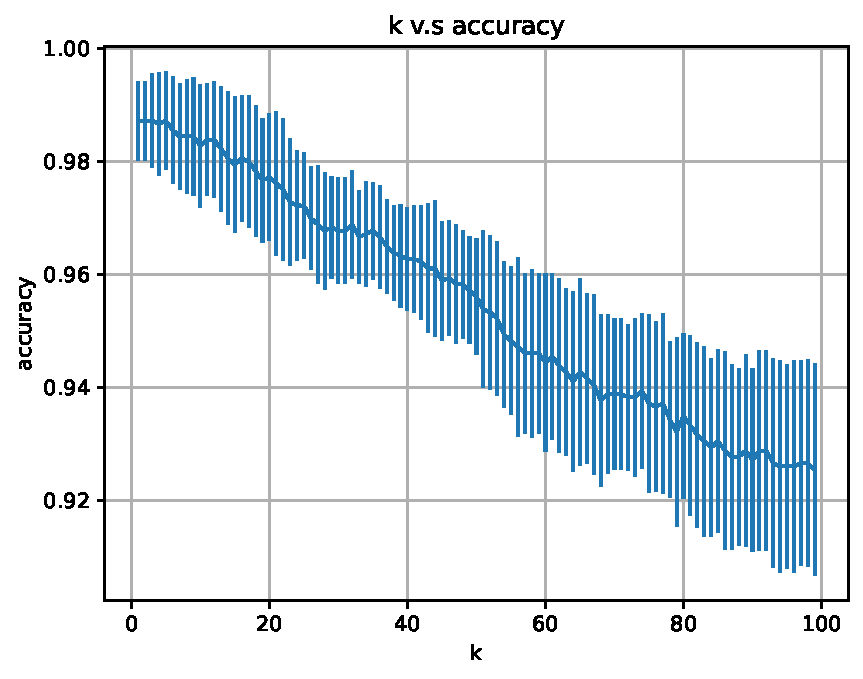
\includegraphics[width=0.30\textwidth]{figures/mnist_knn_accuracy.pdf}
    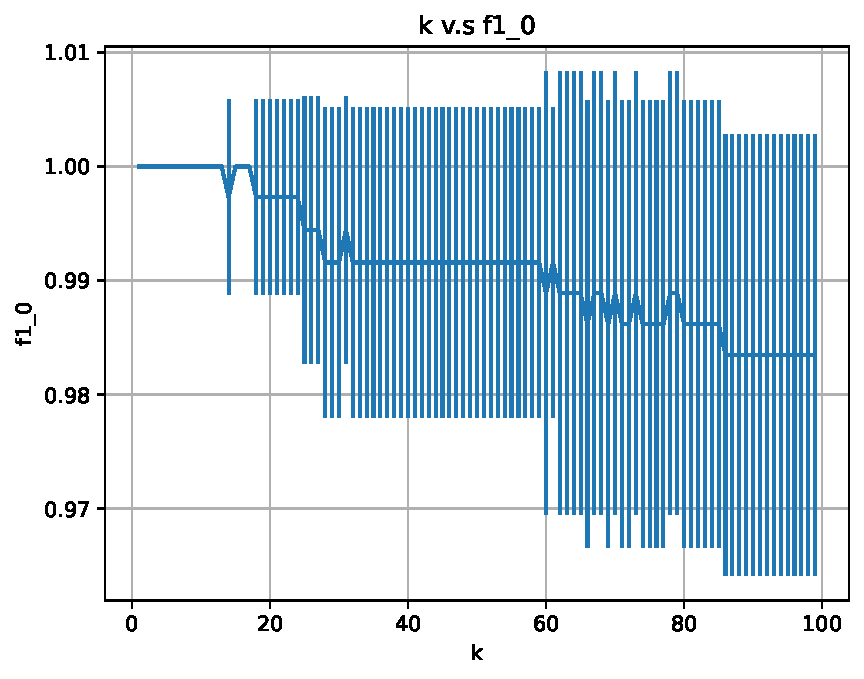
\includegraphics[width=0.30\textwidth]{figures/mnist_knn_f1_0.pdf}
    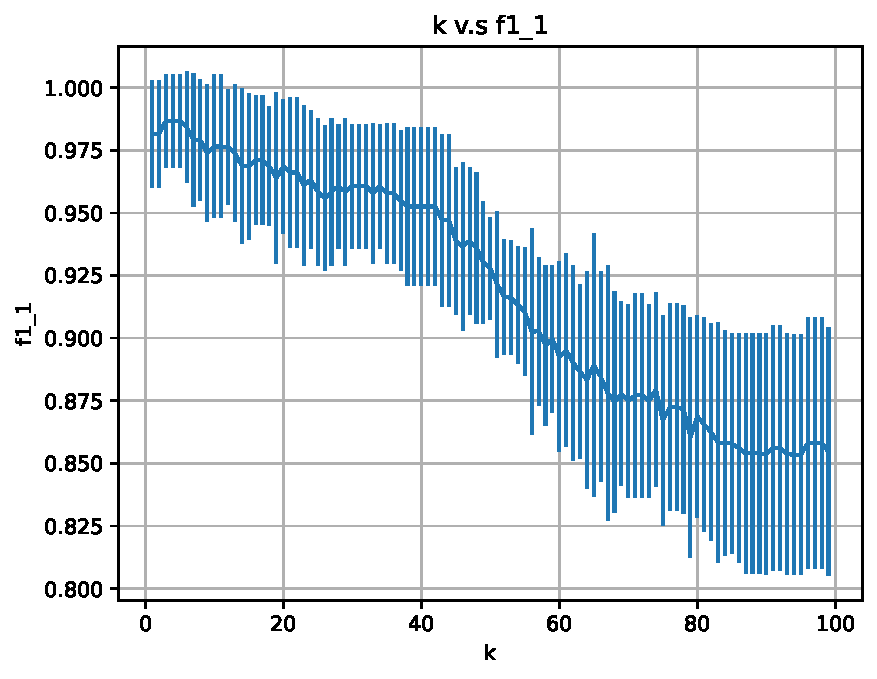
\includegraphics[width=0.30\textwidth]{figures/mnist_knn_f1_1.pdf}
    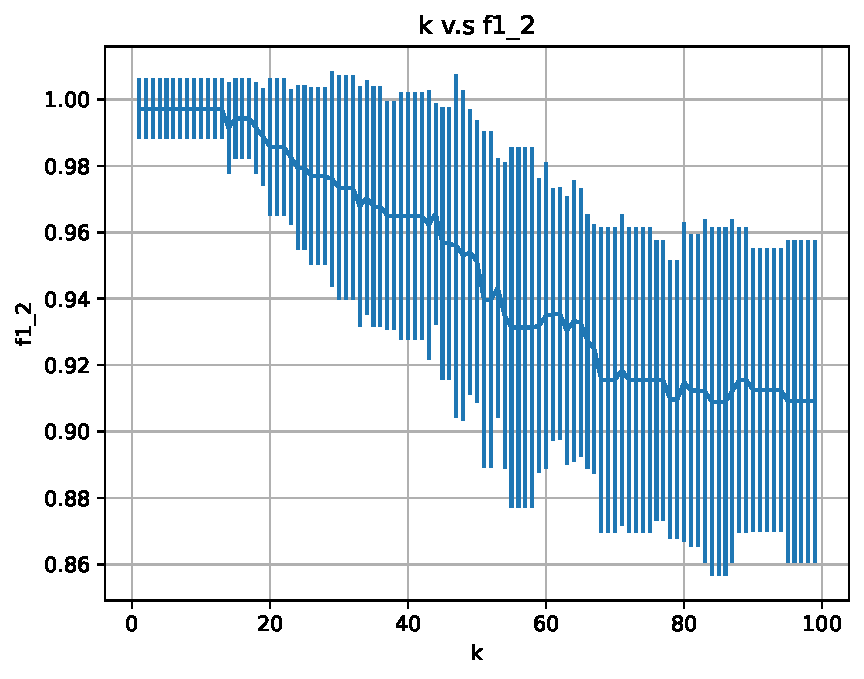
\includegraphics[width=0.30\textwidth]{figures/mnist_knn_f1_2.pdf}
    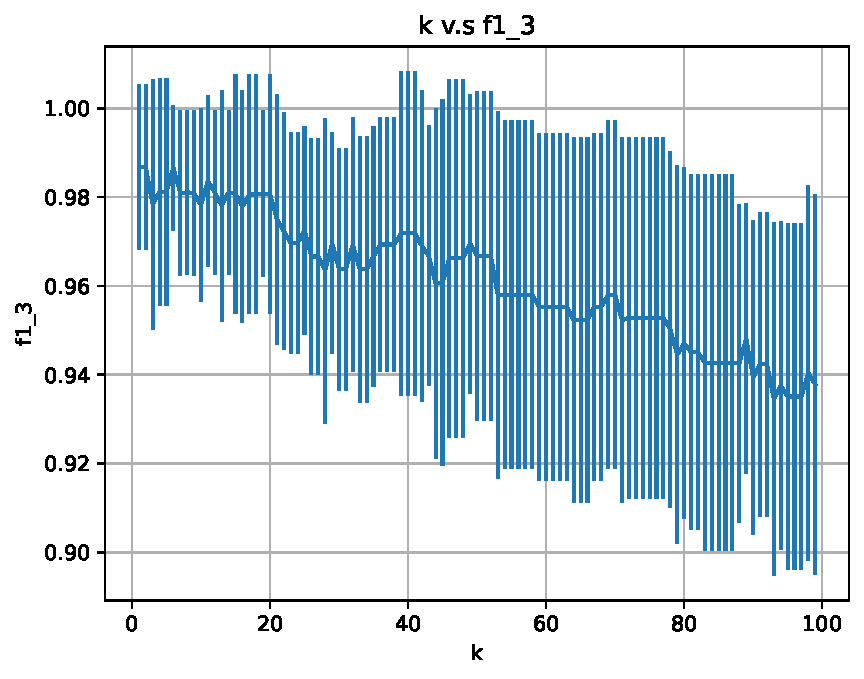
\includegraphics[width=0.30\textwidth]{figures/mnist_knn_f1_3.pdf}
    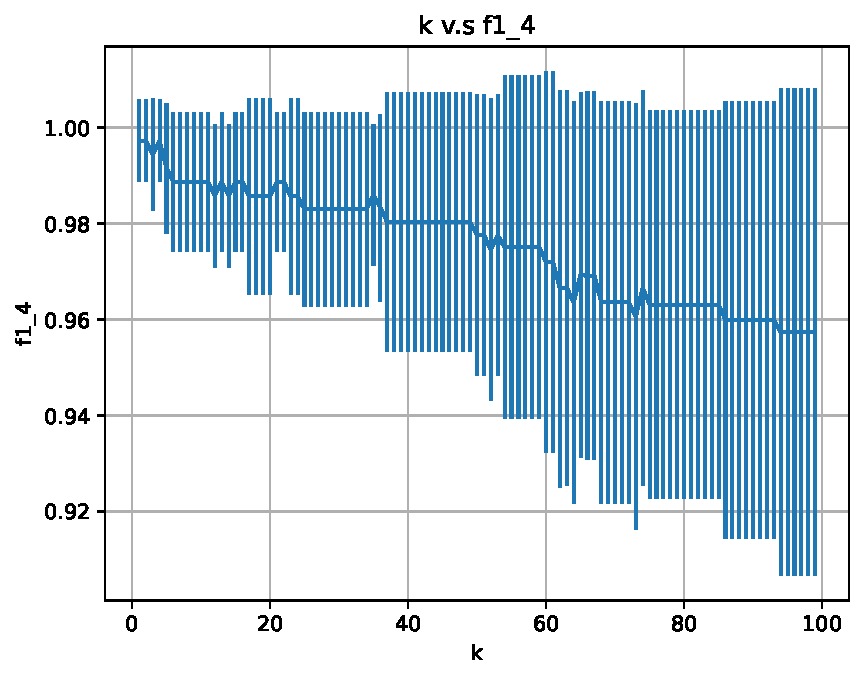
\includegraphics[width=0.30\textwidth]{figures/mnist_knn_f1_4.pdf}
    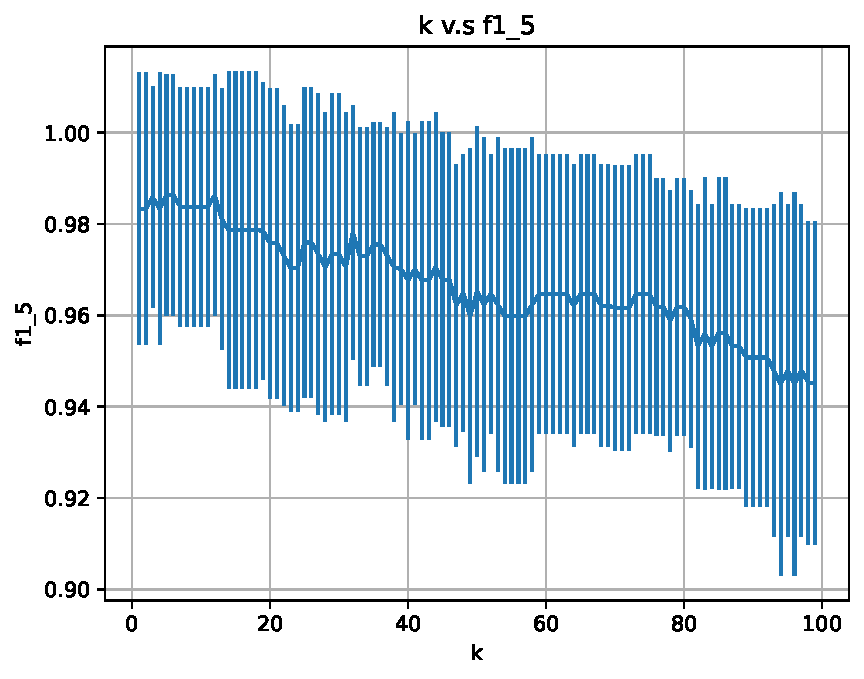
\includegraphics[width=0.30\textwidth]{figures/mnist_knn_f1_5.pdf}
    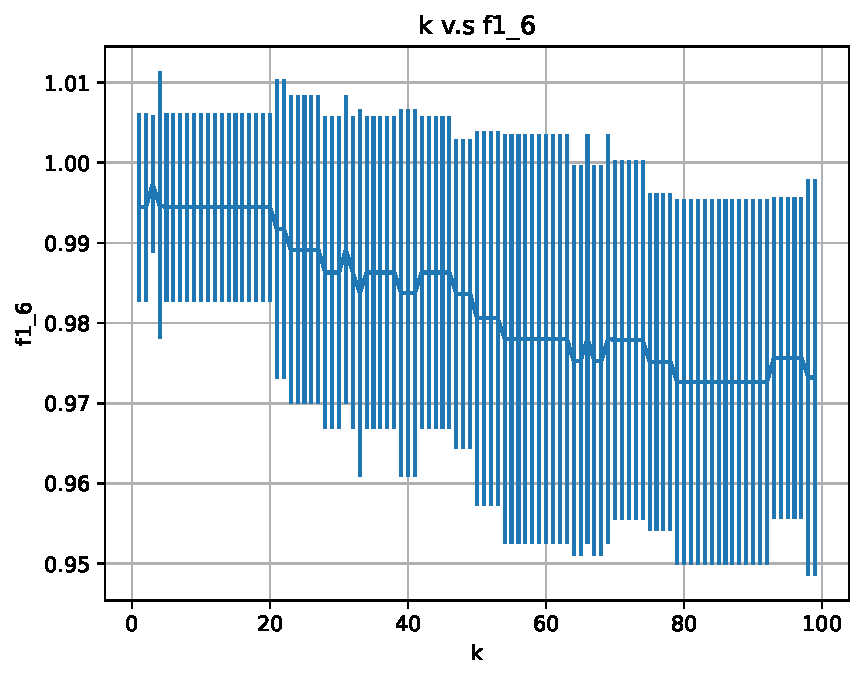
\includegraphics[width=0.30\textwidth]{figures/mnist_knn_f1_6.pdf}
    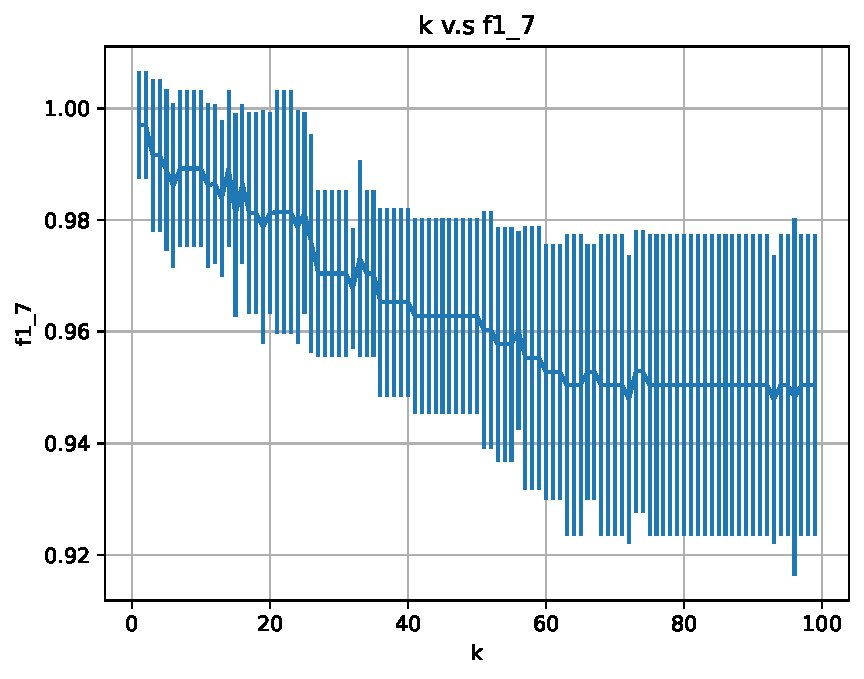
\includegraphics[width=0.30\textwidth]{figures/mnist_knn_f1_7.pdf}
    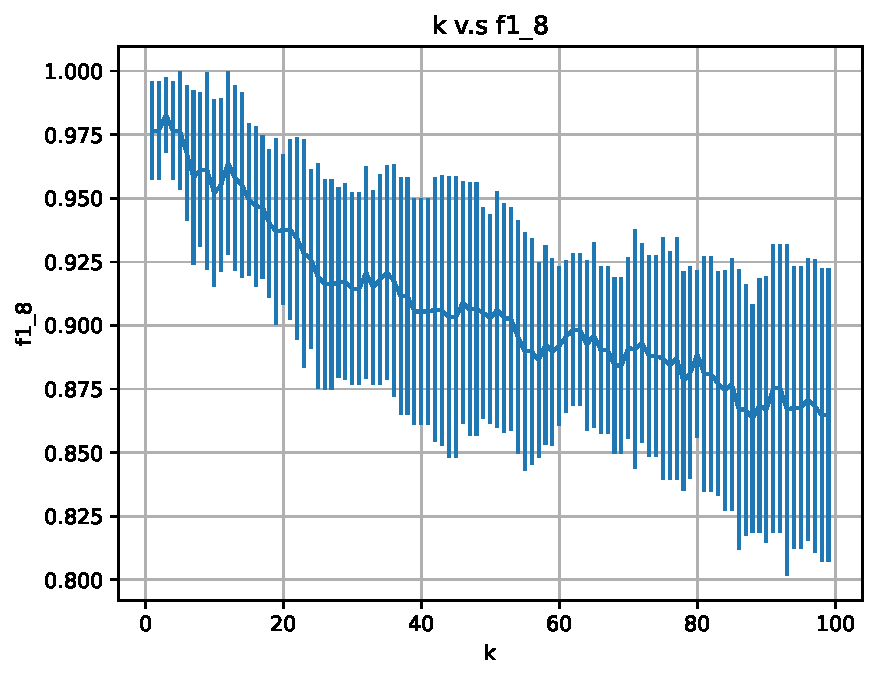
\includegraphics[width=0.30\textwidth]{figures/mnist_knn_f1_8.pdf}
    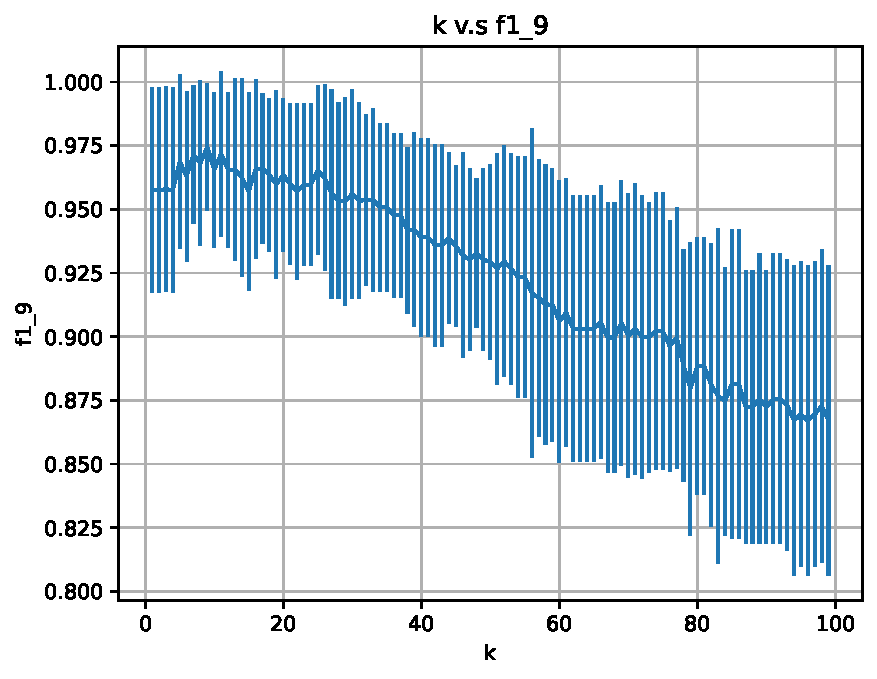
\includegraphics[width=0.30\textwidth]{figures/mnist_knn_f1_9.pdf}
    \caption{Performance metrics graphed against k for KNN on the MNIST dataset.}
    \label{fig:mnist_knn}
\end{figure}

\begin{figure}
    \centering
    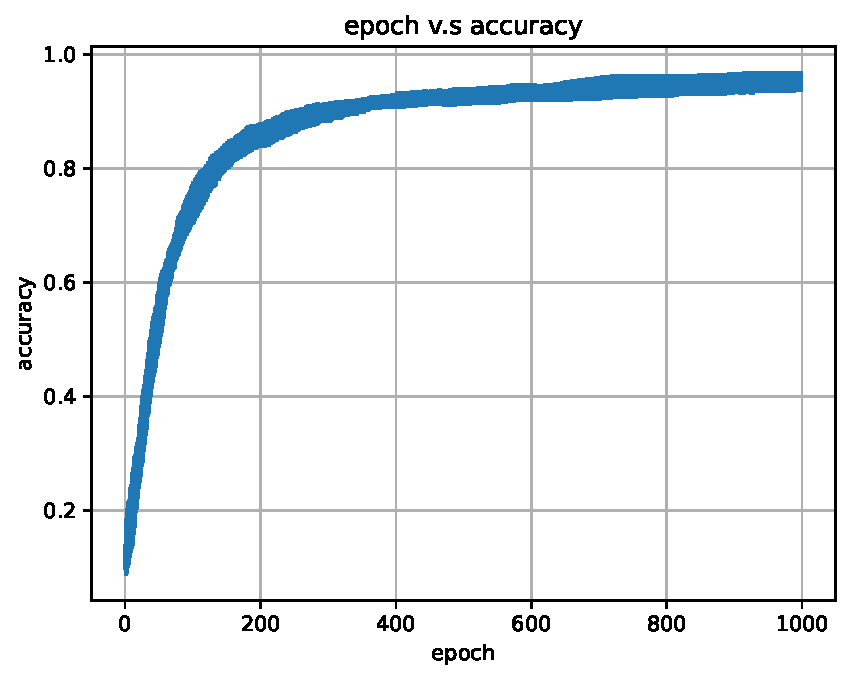
\includegraphics[width=0.30\textwidth]{figures/mnist_nn_accuracy.pdf}
    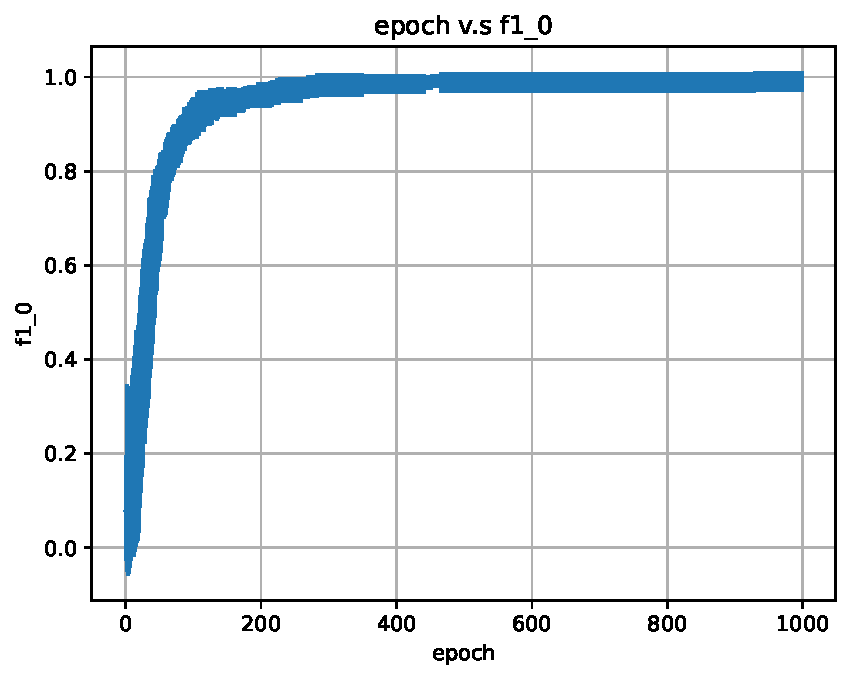
\includegraphics[width=0.30\textwidth]{figures/mnist_nn_f1_0.pdf}
    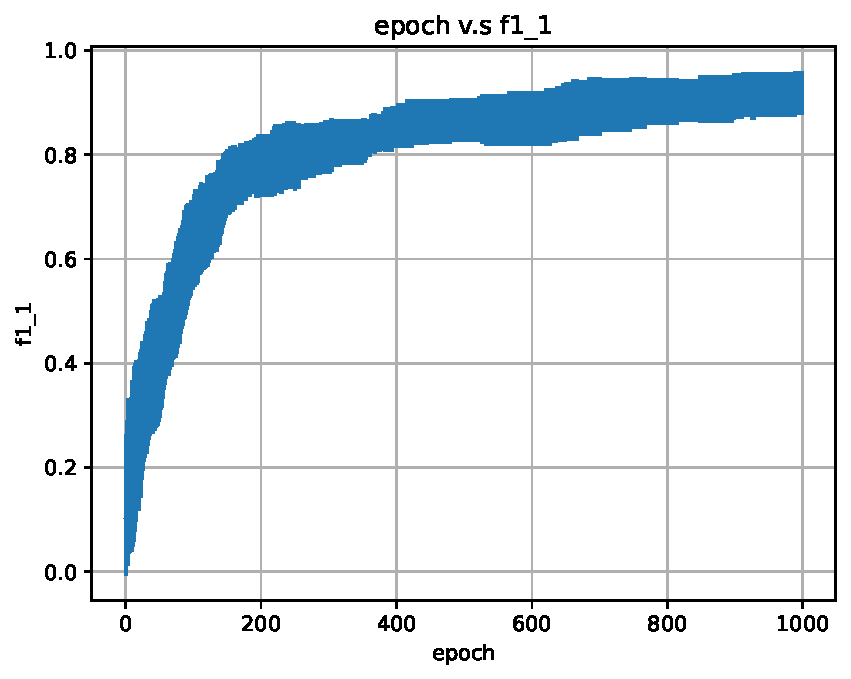
\includegraphics[width=0.30\textwidth]{figures/mnist_nn_f1_1.pdf}
    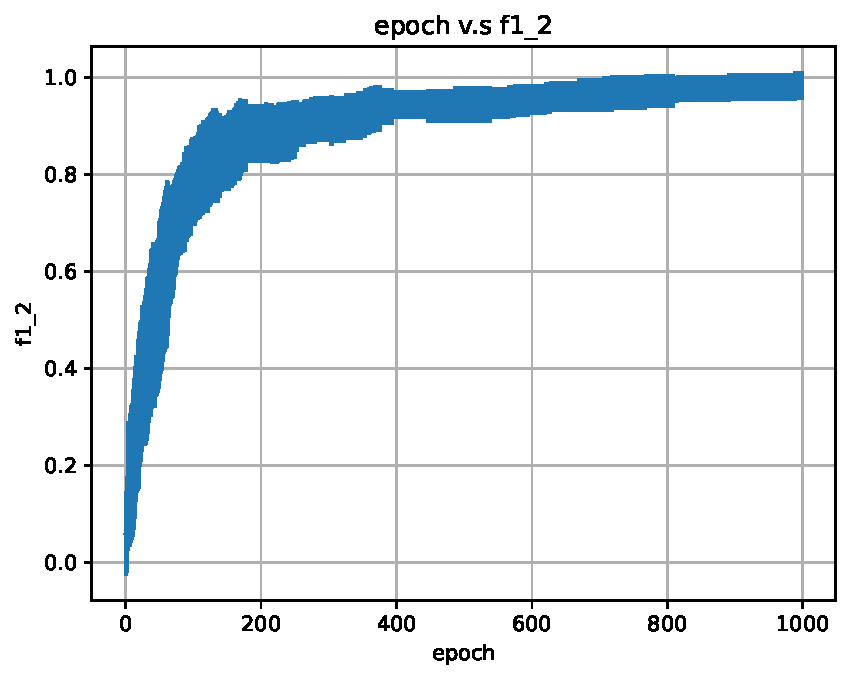
\includegraphics[width=0.30\textwidth]{figures/mnist_nn_f1_2.pdf}
    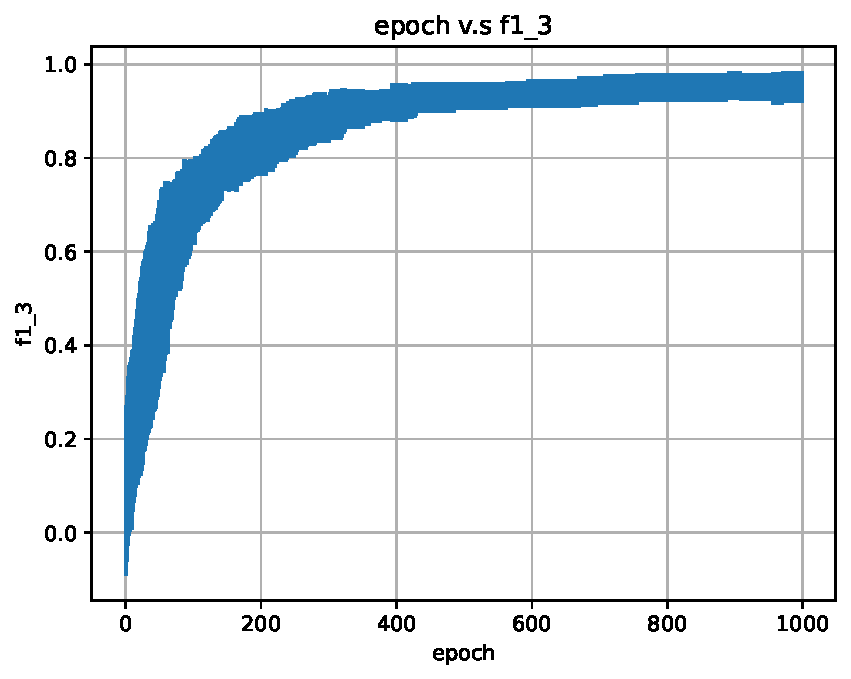
\includegraphics[width=0.30\textwidth]{figures/mnist_nn_f1_3.pdf}
    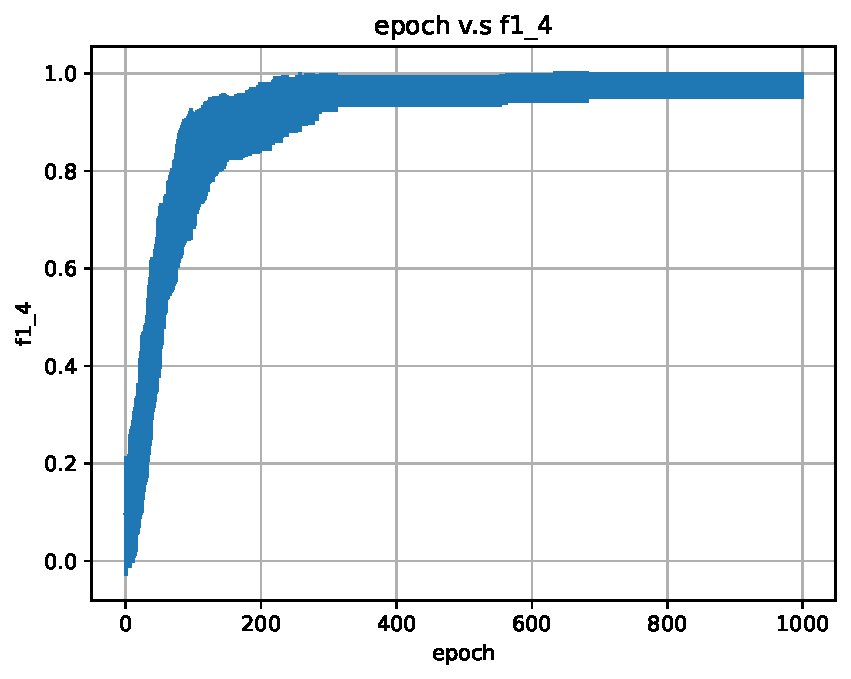
\includegraphics[width=0.30\textwidth]{figures/mnist_nn_f1_4.pdf}
    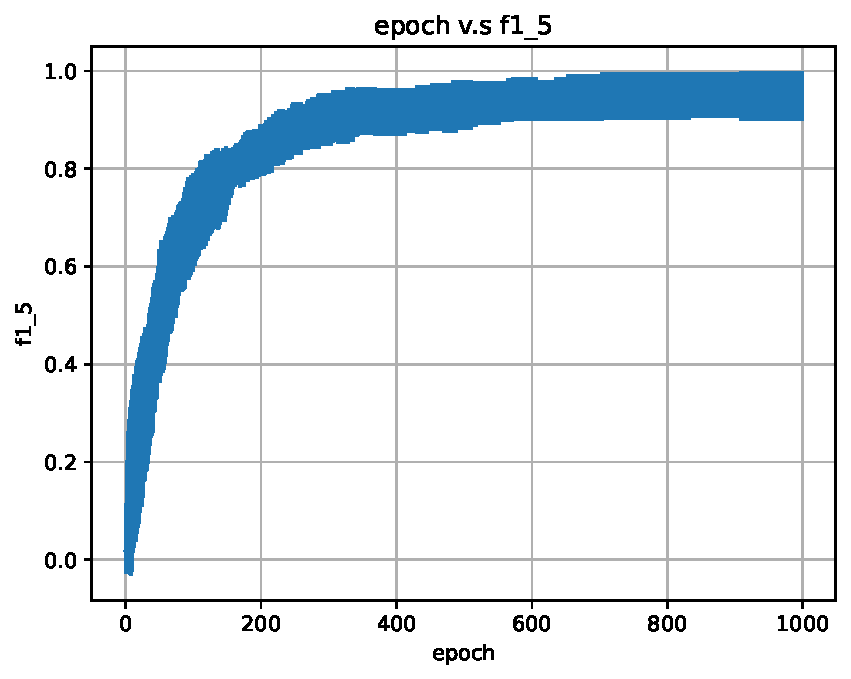
\includegraphics[width=0.30\textwidth]{figures/mnist_nn_f1_5.pdf}
    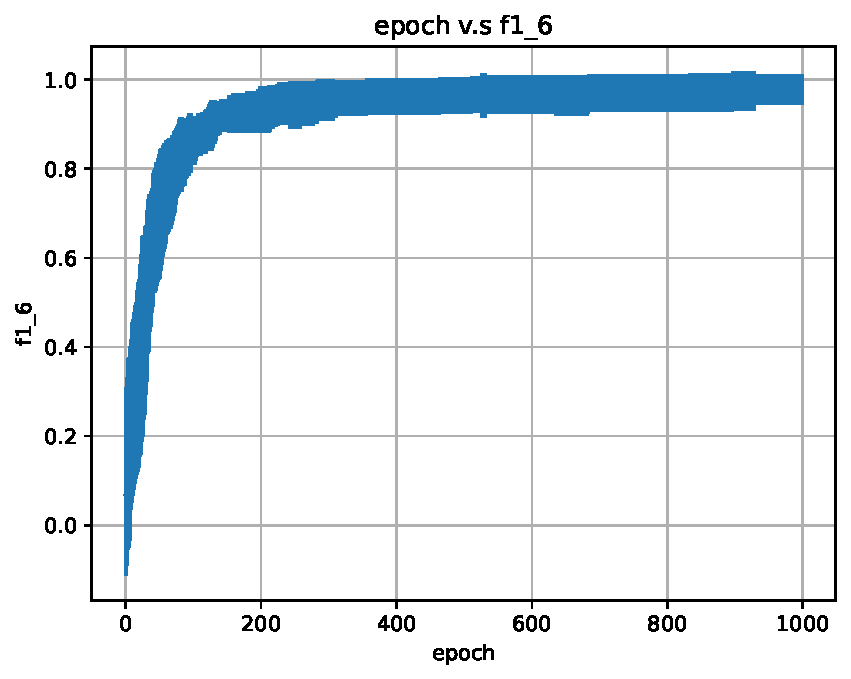
\includegraphics[width=0.30\textwidth]{figures/mnist_nn_f1_6.pdf}
    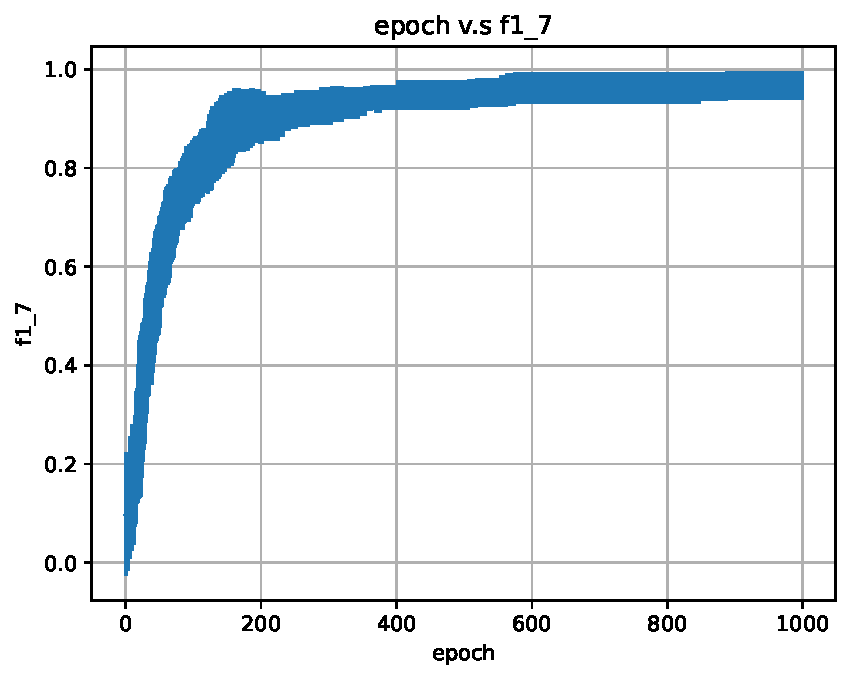
\includegraphics[width=0.30\textwidth]{figures/mnist_nn_f1_7.pdf}
    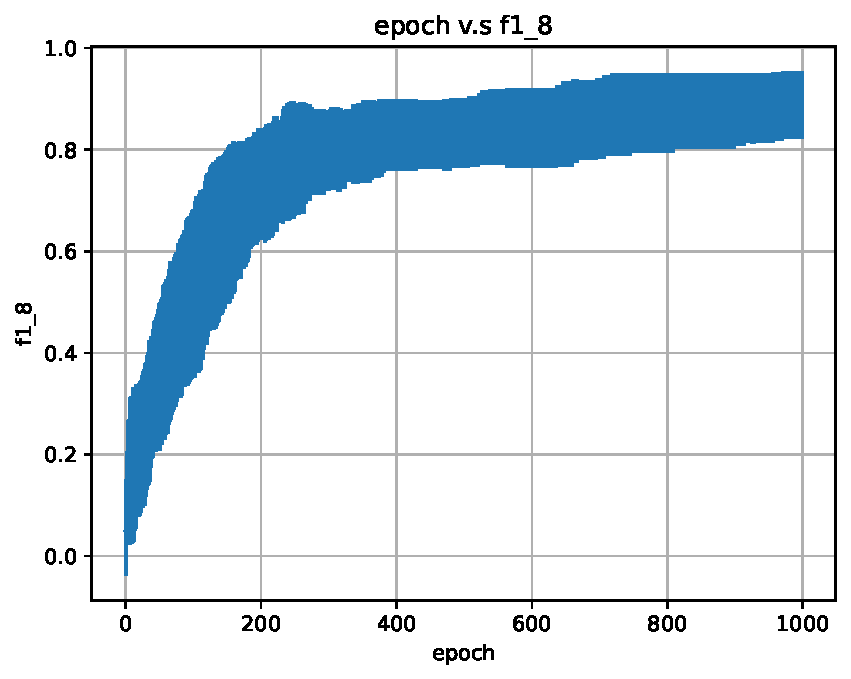
\includegraphics[width=0.30\textwidth]{figures/mnist_nn_f1_8.pdf}
    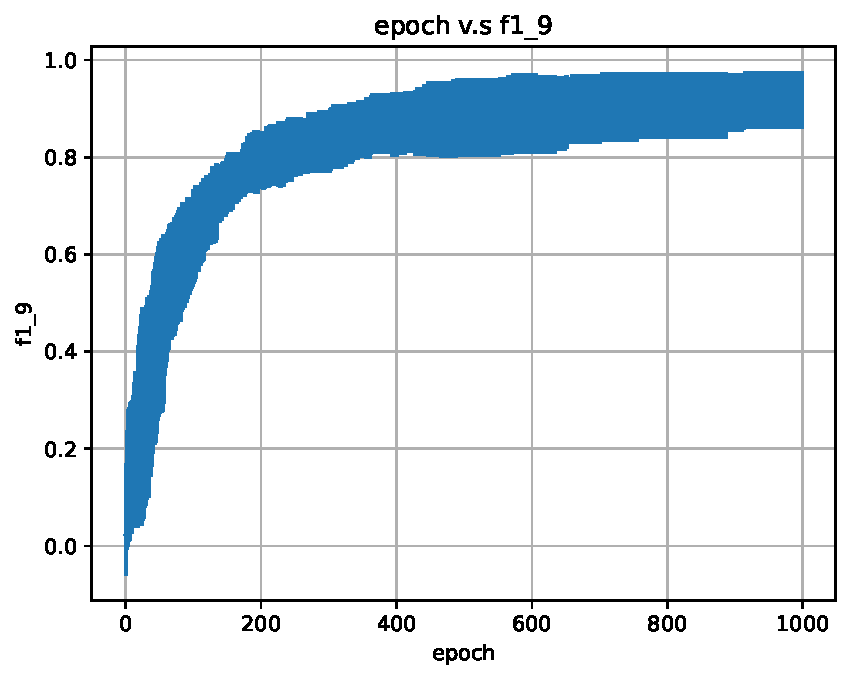
\includegraphics[width=0.30\textwidth]{figures/mnist_nn_f1_9.pdf}
    \caption{Training graphs for a MLP trained on the MNIST dataset.}
    \label{fig:mnist_nn}
\end{figure}

\begin{figure}
    \centering
    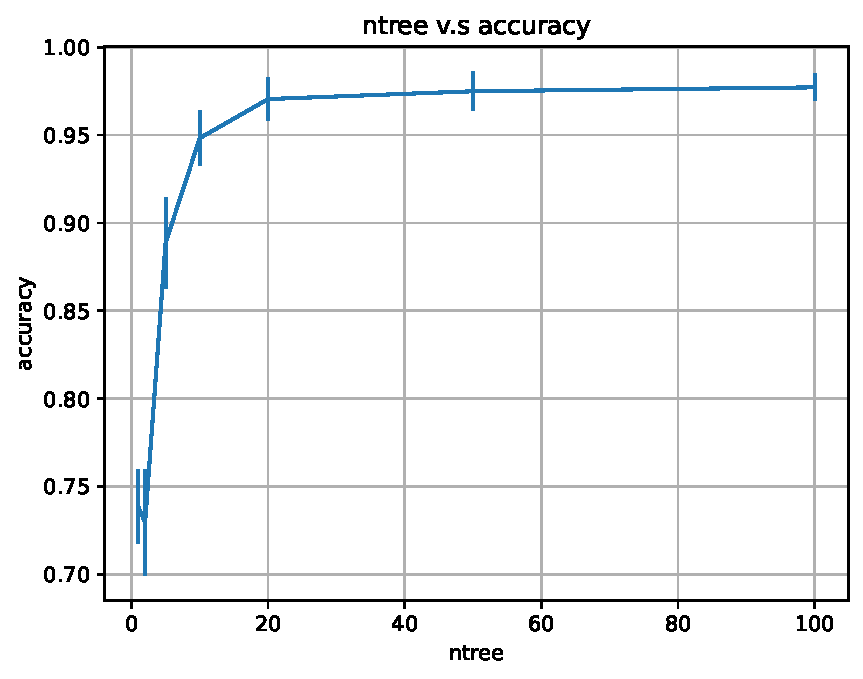
\includegraphics[width=0.30\textwidth]{figures/mnist_random_forest_accuracy.pdf}
    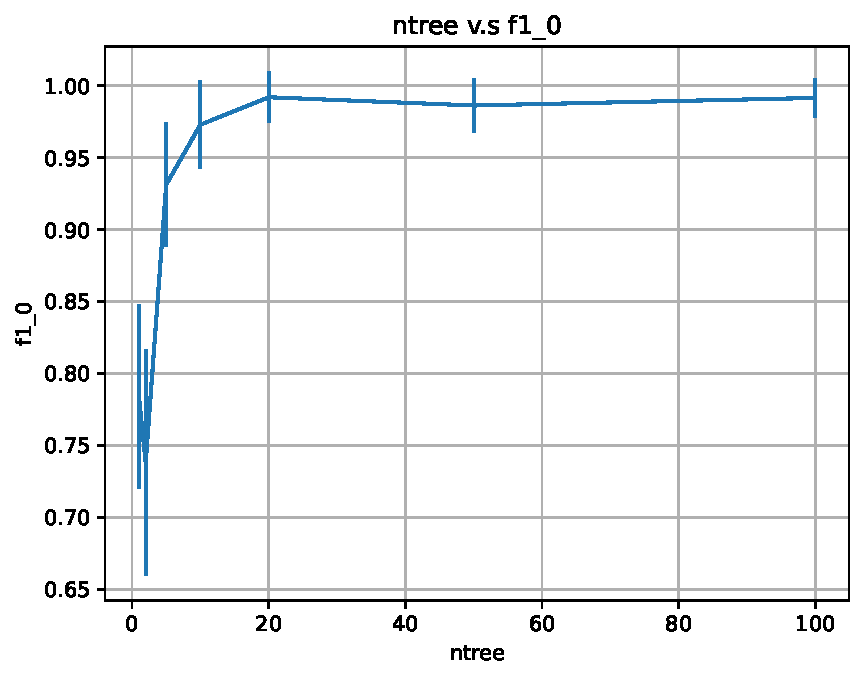
\includegraphics[width=0.30\textwidth]{figures/mnist_random_forest_f1_0.pdf}
    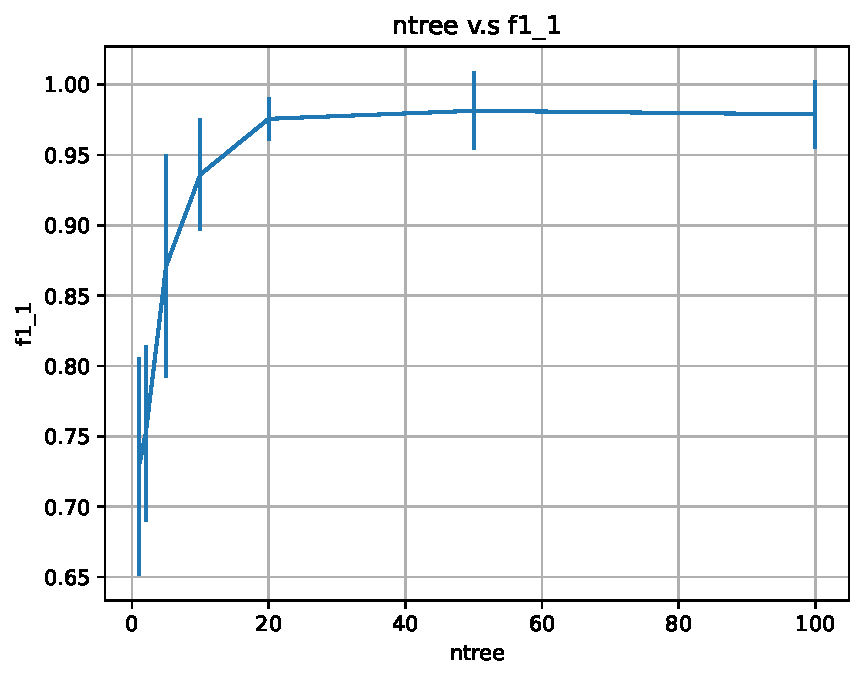
\includegraphics[width=0.30\textwidth]{figures/mnist_random_forest_f1_1.pdf}
    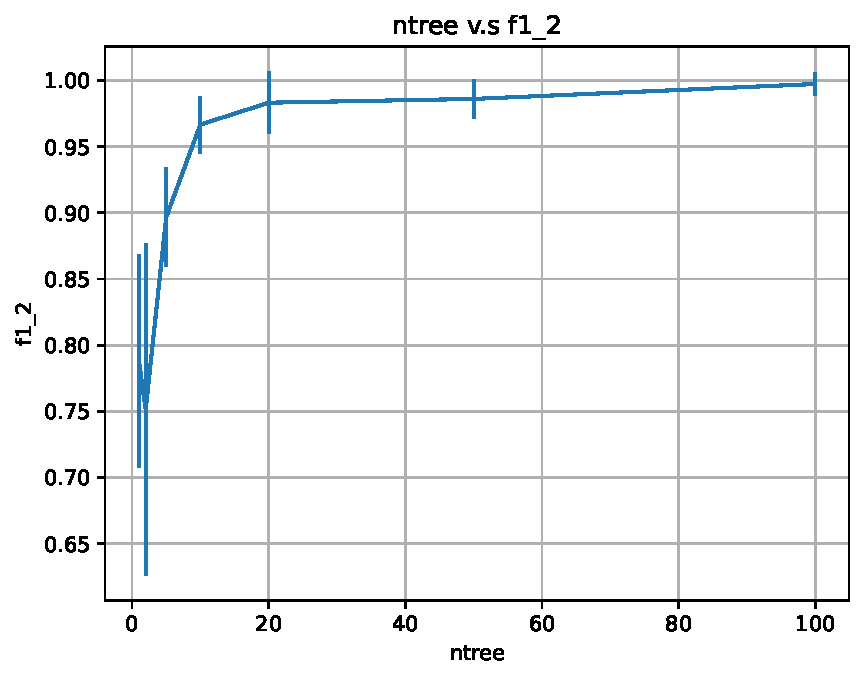
\includegraphics[width=0.30\textwidth]{figures/mnist_random_forest_f1_2.pdf}
    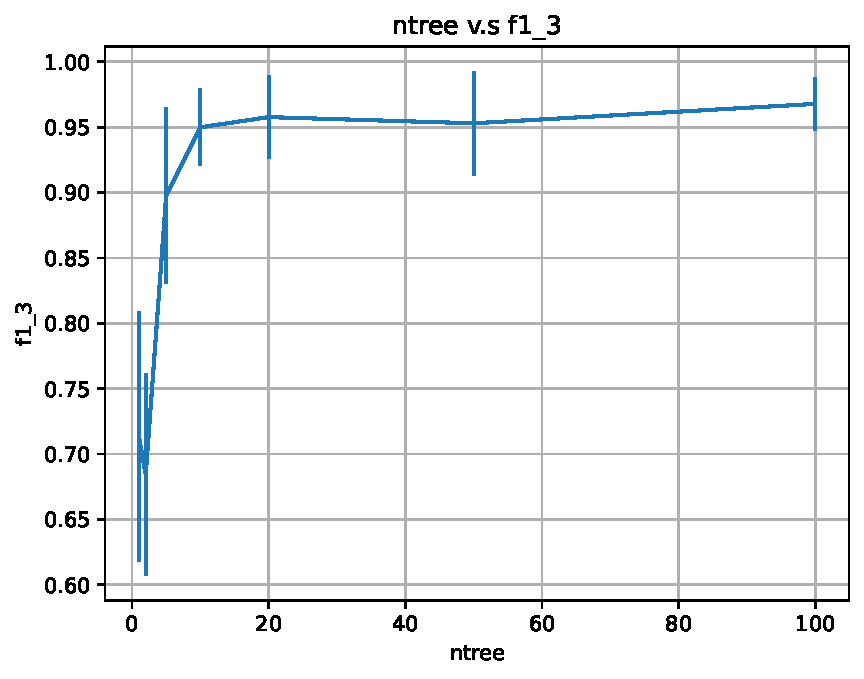
\includegraphics[width=0.30\textwidth]{figures/mnist_random_forest_f1_3.pdf}
    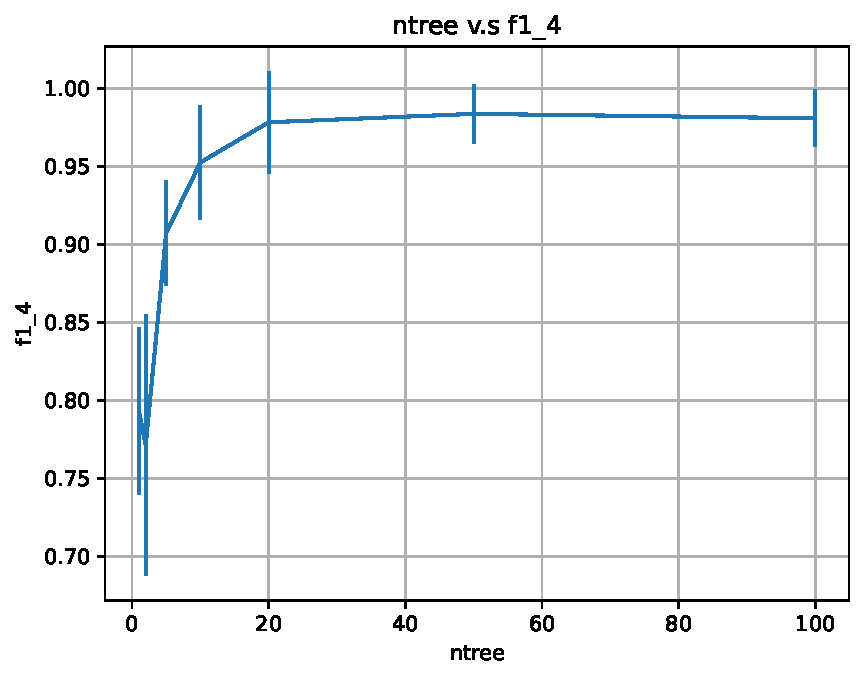
\includegraphics[width=0.30\textwidth]{figures/mnist_random_forest_f1_4.pdf}
    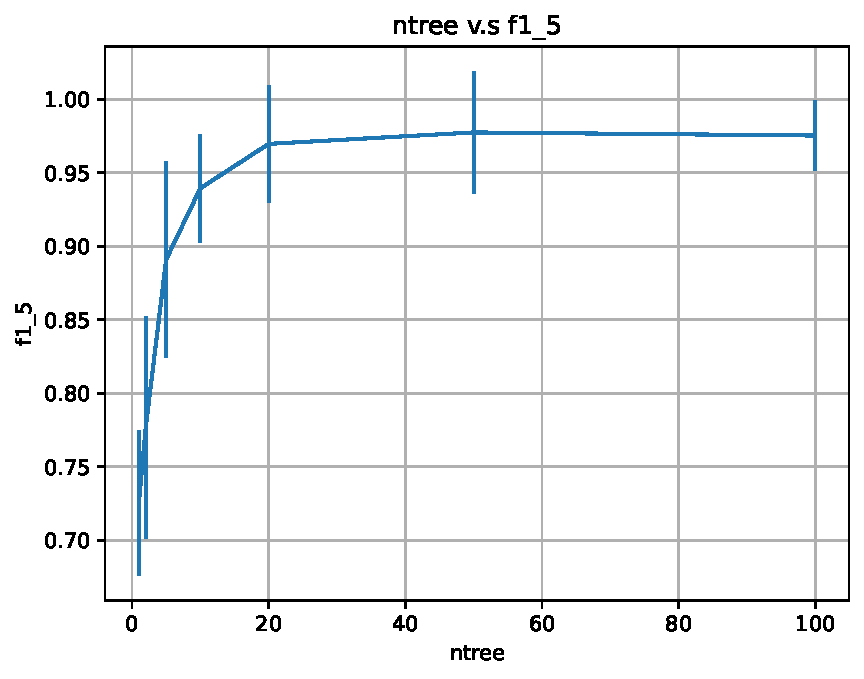
\includegraphics[width=0.30\textwidth]{figures/mnist_random_forest_f1_5.pdf}
    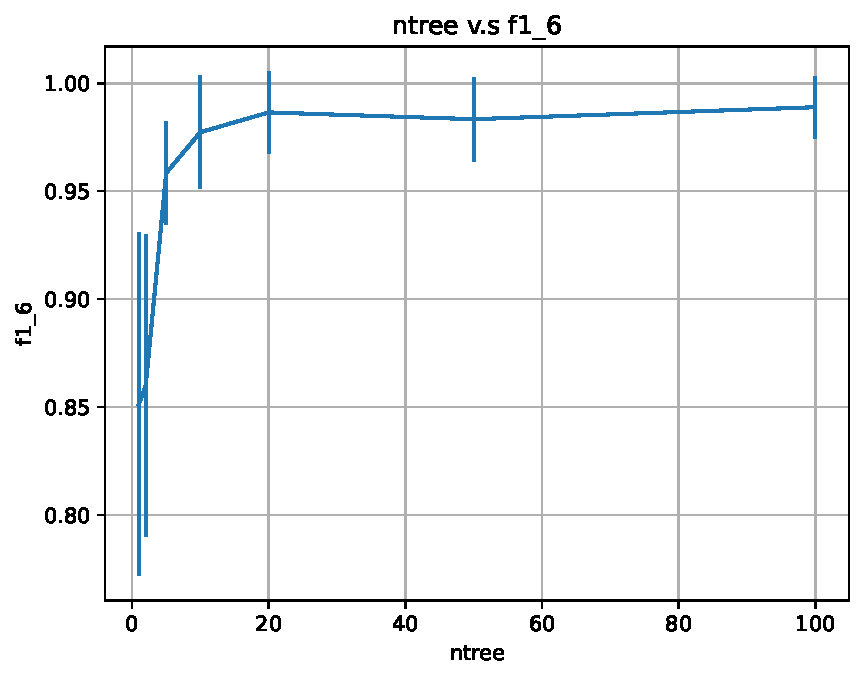
\includegraphics[width=0.30\textwidth]{figures/mnist_random_forest_f1_6.pdf}
    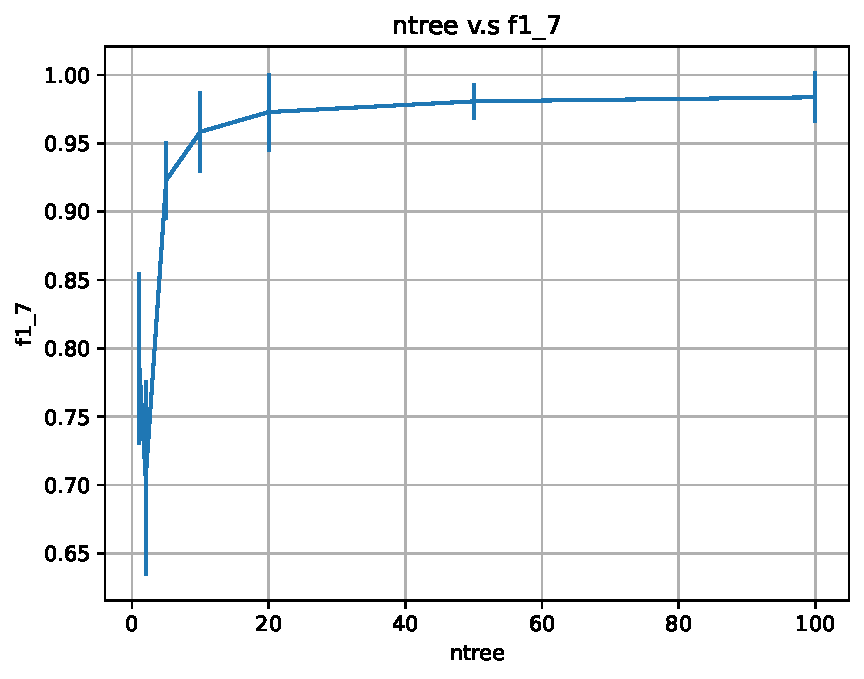
\includegraphics[width=0.30\textwidth]{figures/mnist_random_forest_f1_7.pdf}
    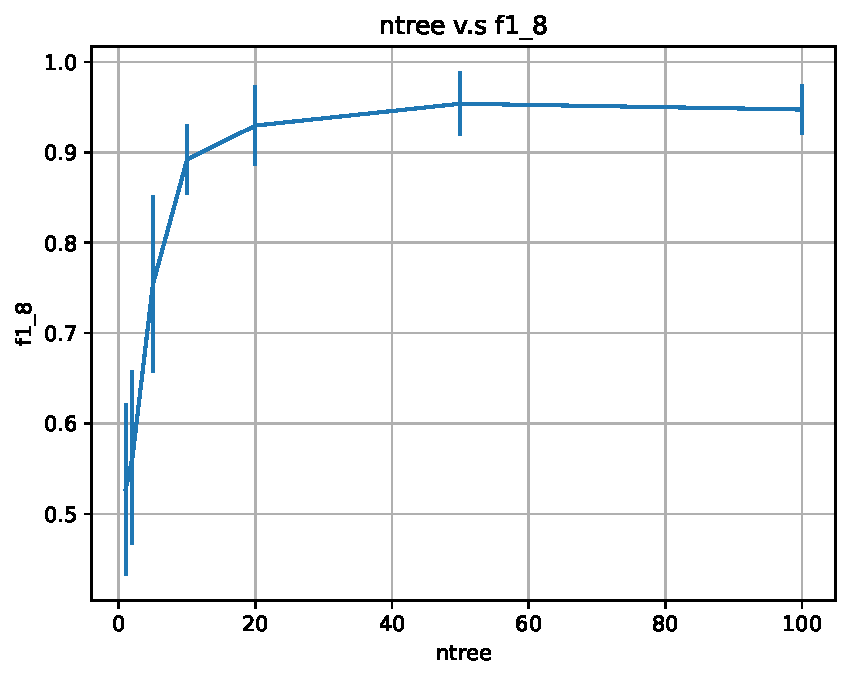
\includegraphics[width=0.30\textwidth]{figures/mnist_random_forest_f1_8.pdf}
    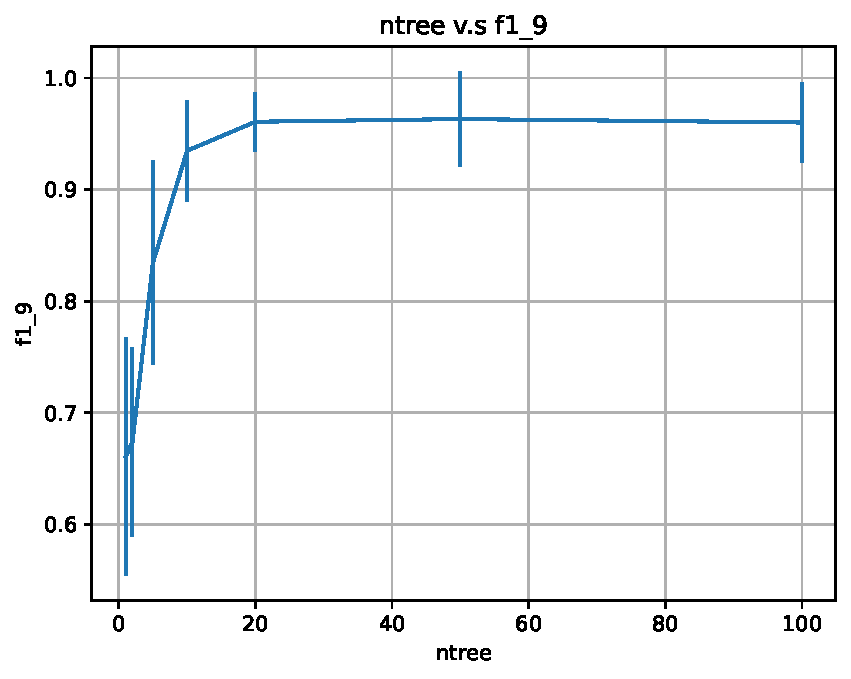
\includegraphics[width=0.30\textwidth]{figures/mnist_random_forest_f1_9.pdf}
    \caption{Performance metrics graphed against ntree for random forests trained on the MNIST
             dataset}
    \label{fig:mnist_random_forest}
\end{figure}
